% Imporditud: tools/import_eksperimendid.py
% Allikas: Eesti füüsikaolümpiaadi eksperimendi ülesannete
%   kogu (Rael Kalda, 2023), ülesanne Ü148, lahendus L148.
\setAuthor{Eero Uustalu}
\setRound{lõppvoor}
\setYear{2017}
\setNumber{P E2}
\setDifficulty{4}
\setTopic{geomeetriline optika}
\setVahendid{Fresneli kumerlääts, Fresneli nõguslääts, mõõtejoonlaud}
\setPunktid{12}
\setAllikas{Eksperimendi kogu Ü148, lahendus lk 110}
\setLahendusseis{toores}

\prob{Läätsed}
Määrake Fresneli nõgusläätse fookuskaugus fn.
\begin{center}
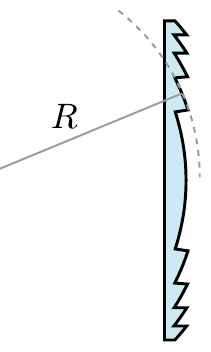
\includegraphics[width=0.20\linewidth]{2017-v3g-pe2-yl.png}
\end{center}
\textit{Näpunäited:} Selles katses kasutatava Fresneli kumerläätse üks pind on tasane ning teine koosneb kaarjatest segmementidest raadiusega R (joonis läbilõikest). Fresneli läätse sakilise pinna võib asendada mõttelise sfäärilise pinnaga, mille kõverusraadius on samuti R, ilma et läätse fookuskaugus sellest muutuks.

\hint

\solu
Leiame kumerläätse fookuskaguuse fk kasutades kaugel asuvat valgusallikat, näiteks laelampi. Asetame kumerläätse ja nõgusläätse ükesteise peale ning leiame liitläätse fookuskauguse fl samal meetodil. Teades, et liitläätse optiline tugevus on üksikute läätsete optiliste tugevuste summa, saame leida nõgusläätse optilise tugevuse ja fookuskauguse fn.

Dl = Dk + Dn $\Rightarrow$ 111 $\Rightarrow$ fn = fk fl =+ fk + fl

fl fk fn
\probend
